% !TEX encoding = UTF-8
% !TEX TS-program = pdflatex
% !TEX root = ../tesi.tex

%**************************************************************
\chapter{Progettazione}
\label{cap:progettazione}
%**************************************************************

% \intro{Breve introduzione al capitolo}\\

% %**************************************************************
\section{Architettura del progetto}
Dato le dimensioni contenute del progetto e per il fatto che deve essere fatta un'analisi 
comparativa con un'altro progetto, si è deciso di strutturarlo con un'architettura a monolite
basata sulla layered architecture.
\\
In questo modo viene velocizzata la realizzazione del progetto, a discapito della facilità di
manutenzione ma non è un problema essendo questo progetto di dimensioni contenute ed in caso
il progetto dovesse crescere fino al punto in cui risulti difficile manutenerlo è sempre possibile
migrarlo in un progetto con un'architettura a microservizi.

% ref: https://cs.uwaterloo.ca/~m2nagapp/courses/CS446/1195/Arch_Design_Activity/Layered.pdf
\subsection{Layered architecture}
La layered architecture è uno degli stili architetturali più utilizzati. L'idea che sta dietro a
questo tipo di architettura è che i moduli o i componenti con funzionalità simili sono organizzati
in livelli orizzontali. Di conseguenza ogni livello svolge un ruolo specifico nell'applicazione.
\\
La layered architecture non ha restrizioni sul numero di strati che l'applicazione può avere, in quanto 
lo scopo è avere livelli che promuovano il concetto di separazione delle responsabilità.
\begin{figure}[!h]
    \centering
    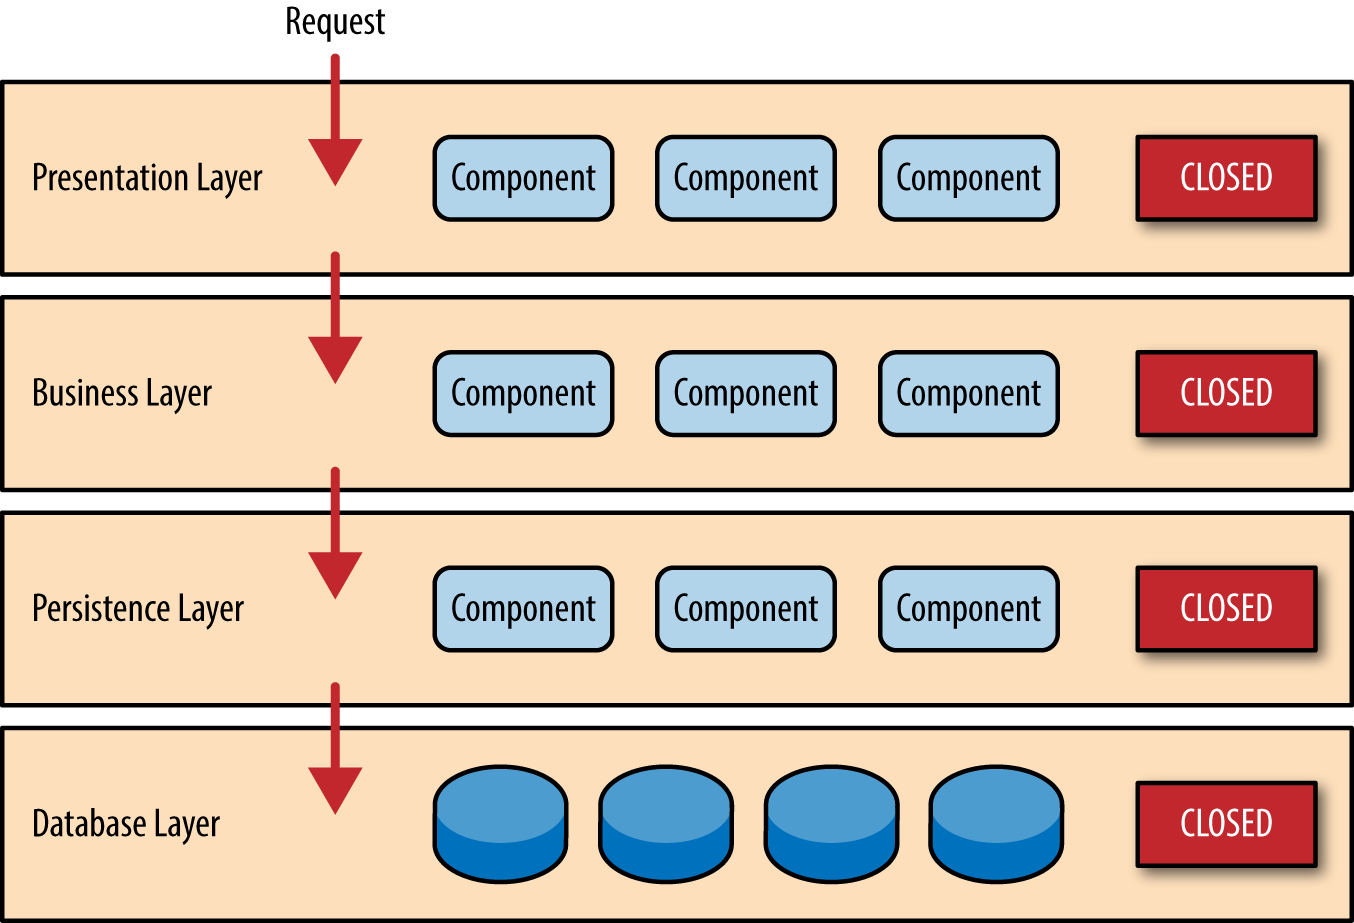
\includegraphics[height=6cm]{layered-architecture}
\end{figure}
\leavevmode\newline
Solitamente ogni livello comunica solo con il livello sottostante. Il connettore tra ogni livello può 
essere una chiamata di funzione, una richiesta di query, un oggetto dati o qualsiasi connettore che
trasmetta richieste o informazioni.
\\
La denominazione dei livelli è abbastanza flessibile ma di solito un livello di presentazione, un livello
di business e un livello fisico sono sempre presenti
\\\\
Livello di presentazione
\\
Il livello di presentazione contiene tutte le classi responsabili di presentare la visualizzazione delle
delle informazioni all'utente finale. Idealmente questo è il solo livello con cui l'utente finale 
interagisce.
\\\\
Livello di business
\\
Il livello di business contiene tutta la logica che è richiesta dall'applicazione per poter soddisfare i 
suoi requisiti funzionali. Solitamente questo livello si occupa dell'aggregazione dei dati, della computazione
e della richiesta dei dati. Quindi qui è dove viene implementata la logica principale dell'applicazione.
\\\\
Livello fisico
\\
Qui è dove sono salvati tutti i dati recuperabili dell'applicazione. Solitamente questo livello è chiamato
anche livello di persistenza. Questo livello si occupa di interagire con il sistema in cui i dati 
sono mantenuti in maniera persistente, come ad esempio un database.
\leavevmode\newline
\subsection{Motivazioni della scelta}
Le motivazione che hanno portato a scegliere questo stile architetturale sono le seguenti:
\begin{itemize}
    \item Dato che la separazione delle responsabilità è la proprietà principale di quest'architettura,
        ogni livello di software ha la sua specifica funzione. Questo rende facile il dover aggiornare 
        singoli livelli e permette al team di sviluppo di separare bene i carichi di lavoro tra i vari 
        membri, che possono lavorare in maniera contemporanea su livelli diversi.
    \item Per la proponente è importante avere una suite di test automatici per testare i vari componenti
        dell'applicazione. La layered architecture separando bene le responsabilità tra i livelli, 
        permette di suddividere l'applicazione in componenti ben separati e quindi più facili da testare.
        Essendo ogni livello isolato dagli altri, è possibile creare casi di test di dimensione ridotta, 
        in quanto le componenti di cui fare il mock sono poche.
    \item L'isolamento tra i vari livelli permette di modificare un livello senza che la modifica intacchi
        gli altri livelli.
    \item Nel caso l'applicazione diventi molto grande è possibile senza troppo sforzo avviare un processo
        di migrazione ad un'architettura a microservizi. La layered architecture lavora bene come monolite 
        in un sistema con un'architettura ibrida tra un monolite e un sistema a microservizi. Questa architettura
        ibrida andrà a formarsi nel mentre che il monolite viene migrato in un sistema a microservizi, quindi 
        è importante avere un architettura a monolite che lavori bene in questo tipo di sistema.
        \\
        Inoltre grazie alla separazione delle responsabilità della layered architecture è più facile andare
        a trasformare i componenti del monolite in microservizi.
\end{itemize}

\section{Struttura software}
E' stato scelto NestJS come framework di sviluppo del progetto dato che si adatta bene con la layered architecture,
dato che usa il pattern controller-service-repository, un pattern basato sulla layered architecture,  
per permettere allo sviluppatore di sviluppare le proprie applicazioni.
\begin{figure}[!h]
    \centering
    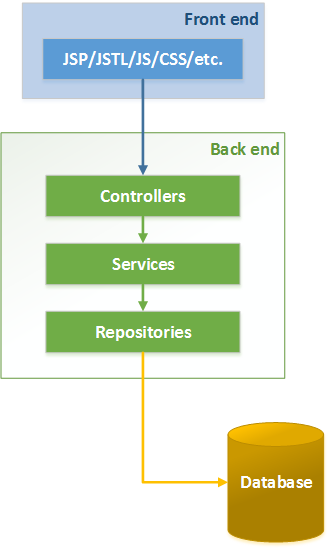
\includegraphics[height=6cm]{controller-service-repository-pattern}
\end{figure}
\leavevmode\newline
Il controller è il livello responsabile per gestire le richieste in arrivo e ritornare le risposte al client.
Esiste un meccanismo di routing che gestisce a quale controller inviare le richieste.
\\
Il service è il livello responsabile della business logic.
\\
Il repository è il livello chiamato livello di persistenza nella layered architecture.
\\\\
Analizziamo in dettaglio la struttura del software:

\subsection{IoC container}
L'Inversion of Control container è un componente fondamentale di NestJS che permette l'applicabilità
del pattern Dependency Injection all'interno di NestJS.
\\
L'IoC container contiene un'istanza di tipo singleton per ogni classe dichiarata come controller o provider.
\\\\
Il funzionamento dell'IoC container è il seguente:
\\
quando viene avviata un'applicazione NestJS, il sistema runtime ricerca tutti controller e provider che 
sono stati dichiarati in dei moduli importati dal modulo root. Per ognuna di queste classi crea un'istanza
usando il pattern singleton e la inserisce nell'IoC container. 
\\
Se però la classe da istanziare dichiarava una dipendenza con un altro controller o provider nel proprio 
costruttore, il sistema runtime applica in maniera automatica il pattern Dependency Injection; ovvero
va a cercare un'istanza della dipendenza dichiarata nel costruttore della classe nell'IoC container, se
presente la inietta nella classe e crea l'istanza della nuova classe da inserire nell'IoC container. 
\\
Altrimenti va a creare
l'istanza della classe che deve essere iniettata, prima della classe che dichiara la dipendenza (se possibile, in quanto la
classe da iniettare potrebbe a sua volta richiedere una dipendenza e in tal caso si segue la successione di 
dipendenze fino a che non si trova una classe che possa essere istanziata) e la inietta nella classe che dichiara
la dipendenza, poi ne crea un'istanza e la inserisce nell'IoC container.

\subsection{Controller e provider}
I due componenti fondamentali di NestJS sono i controller e i provider. 
Per dichiarare una classe come controller, bisogna applicare il decorator @Controller, sopra la 
definizione della classe, mentre per dichiarare una classe come provider bisogna applicare il decorator
@Injectable sopra la definizione della classe.
\\
\begin{lstlisting}
@Injectable()
export class MaintainersRegistryService {
    constructor(private readonly maintainersRegistryRepository: 
        MaintainersRegistryRepository){}

    getAllMaintainers(){
        return this.maintainersRegistryRepository.find();
    }

    async getMaintainerById(id: string){
        const maintainer = 
            await this.maintainersRegistryRepository.findOne({
                where: {
                    id: id
                }
            });

        if(isEmpty(maintainer))
            throw new NotFoundError('maintainer id not found');

        return maintainer;
    }

    async createMaintainer(maintainer: MaintainerRegistry){
        const insertResponse = 
            await this.maintainersRegistryRepository.insert(maintainer);

        if(isEmpty(insertResponse.identifiers))
            throw new InsertError('problem to insert record');

        const maintainerInsertedId = insertResponse.identifiers[0].id;

        return this.getMaintainerById(maintainerInsertedId);
    }

    async editMaintainerById(id: string, maintainerRegistry: MaintainerRegistry){
        try{
            await this.getMaintainerById(id);    
        }catch(error){
            throw(error);
        }
        
        const updateResponse = 
            await this.maintainersRegistryRepository.update(id, maintainerRegistry);

        const numberRowAffected = updateResponse.affected;

        if(numberRowAffected !== 1)
            throw new UpdateError('problem to update record');

        return this.getMaintainerById(id);
    }

    async deleteMaintainerById(id: string){
        try{
            await this.getMaintainerById(id);    
        }catch(error){
            throw(error);
        }

        const deleteResponse = 
            await this.maintainersRegistryRepository.delete(id);

        const numberRowAffected = deleteResponse.affected;

        if(numberRowAffected !== 1)
            throw new DeleteError('problem to delete record');
    }
}
\end{lstlisting}
\leavevmode\newline
\\
I controller sono i componenti dedicati a gestire le richieste in ingresso e a fornire le risposte all'utente
finale. NestJS considera come provider tutte le classi istanziabili e marcate con il decorator 
@Injectable che non sono controller; quindi sia classi di tipo service, che repository devono essere marcate
con il decorator @Injectable. 
\\
\begin{lstlisting}
@Controller('maintainers')
export class MaintainersRegistryController {
    constructor(private readonly maintainersRegistryService: 
        MaintainersRegistryService){}

    @Get()
    getAllMaintainers(){
        return this.maintainersRegistryService
            .getAllMaintainers();
    }

    @Get(':id')
    getMaintainerById(@Param('id') id: string){
        return this.maintainersRegistryService
            .getMaintainerById(id);
    }

    @Post()
    async createMaintainer(@Body() maintainer: MaintainerRegistry){
        return await this.maintainersRegistryService
            .createMaintainer(maintainer);
    }

    @Put(':id')
    editMaintainerById(
        @Param('id') id: string,
        @Body() maintainerRegistry: MaintainerRegistry,
    ){
        return this.maintainersRegistryService
            .editMaintainerById(id, maintainerRegistry);
    }

    @Delete(':id')
    @HttpCode(204)
    deleteMaintainerById(@Param('id') id: string){
        return this.maintainersRegistryService
            .deleteMaintainerById(id);
    }
}
\end{lstlisting}
\leavevmode\newline
\\
E' possibile marcare con il decorator @Injectable
anche classi non service o repository di cui si vuole che NestJS si occupi
in maniera automatica di istanziare, iniettare le dipendenze dichiarate nel costruttore e inserire nell'IoC 
container.
\\\\
I controller individuati sono i seguenti:
\begin{itemize}
    \item MaintainersRegistryController: gestisce le richieste/risposte relative al dominio dei manutentori.
    \item ParkingAreasController: gestisce le richieste/risposte relative al dominio dei parcheggi.
    \item ParkingSensorsController: gestisce le richieste/risposte relative al dominio delle misurazioni
    dei sensori di parcheggio.
    \item ParkingSensorsSensorsController: gestisce le richieste/risposte relative al dominio delle misurazioni
    dei sensori di parcheggio di un sensore.
    \item ParkingSpotsController: gestisce le richieste/risposte relative al dominio delle piazzole.
    \item ParkingSpotsParkingAreasController: gestisce le richieste/risposte relative al dominio delle piazzole
    di un parcheggio.
    \item ParkingSpotsSensorsController: gestisce le richieste/risposte relative al dominio delle piazzole
    di un sensore.
    \item SensorsController: gestisce le richieste/risposte relative al dominio dei sensori.
    \item SensorsParkingSpotsController: gestisce le richieste/risposte relative al dominio dei sensori di una
    piazzola.
    \item SensorsMaintenanceSensorsController: gestisce le richieste/risposte relative al dominio della manutenzione dei
    sensori di un sensore.
\end{itemize}

\subsection{Repository}
I repository sono i componenti dedicati alla gestione della persistenza dei dati. Hanno quindi il compito di
comunicare con la componente di archiviazione dati come un database. Nel progetto è stato utilizzato un database
relazionale di tipo postgreSQL.
\\\\
NestJS è indipendente dal tipo di database scelto (relazionale o non relazionale). Infatti NestJS si interfaccia
al database tramite uno strumento che si chiama TypeORM. TypeORM implementa una tecnica di programmazione chiamata 
ORM che converte i dati tra diversi tipi di sistemi usando linguaggi di programmazione OOP.
\\\\
Uno strumento ORM incapsula il codice necessario per manipolare i dati, senza aver bisogno di scrivere manualmente
le query al database ma si interagisce direttamente con un oggetto nello stesso linguaggio che si sta usando. 
\\
In questo modo il database viene astratto e si diventa indipendenti dal tipo di database utilizzato, in quanto è compito dell'ORM
tradurre la richiesta fatta in linguaggio di programmazione ad alto livello nella query al database. 
\\\\
Uno strumento come TypeORM offre quindi una grande flessibilità in quanto è possibile decidere di passare da un database
relazionale a un database non relazionale in qualsiasi momento senza dover effettuare modifiche al livello di persistenza.
\\\\
Senza un'ORM la migrazione da un database relazionale a un database non relazionale implica la riscrittura di tutte le query.
\\\\
Il repository viene fornito e creato in maniera automatica da NestJS. Per fare in modo che ciò avvenga però è necessario
dichiarare, all'interno del modulo in cui si vuole che NestJS crei il repository, nell'array di imports tramite 
il metodo forFeature della classe TypeOrmModule la lista di entità di cui si vuole creare un repository.
\\\\
Il repository creato da NestJS include tutti i metodi necessari per le operazioni basilari CRUD (find(), save(), update(), 
delete() ecc..).
\\\\
Spesso però abbiamo bisogno di effettuare query al database più complesse rispetto a quelle a disposizione nel repository
creato da NestJS. Per fare ciò dobbiamo creare una nostra classe repository che estenda la classe Repository, che è una
classe Generics definita all'interno di NestJS e si aspetta come tipo del Generic il tipo dell'entità di cui vogliamo 
creare il repository.
\\\\
Creato il repository custom non è più necessario usare il metodo forFeature nella classe modulo, ma va importato il repository custom
come provider.
\\ 

\begin{lstlisting}
@Injectable()
export class SensorsRepository extends Repository<Sensor>{
    constructor(private dataSource: DataSource){
        super(Sensor, dataSource.createEntityManager());
    }

    getSensorsWithoutSensorMaintenance(){
        return this.dataSource
        .createQueryBuilder()
        .select('sensor')
        .from(Sensor, 'sensor')
        .leftJoin('sensor.sensorMaintenance', 'sensorMaintenance')
        .where('sensorMaintenance.id IS NULL')
        .getMany();
    }
}
\end{lstlisting}
\leavevmode\newline
Nel nostro repository oltre che ai metodi ereditati dalla classe padre Repository, possiamo creare i nostri metodi personalizzati
per poter inserire le nostre query custom. 
\\\\
Ci sono 2 modi per creare le query:
\begin{itemize}
    \item tramite notazione pura SQL 
    \item tramite i metodi del Query Builder
\end{itemize}
\leavevmode\newline
E' fortemente consigliato l'utilizzo del Query Builder anziché usare la notazione SQL per 2 motivi:
\begin{enumerate}
    \item La concatenazione dei metodi del Query Builder rende molto più chiaro e pulito il codice, quindi più facile
        da manutenere.
    \item Nel caso di cambio di tipo di database le query continuano a funzionare, in quanto grazie al Query Builder,
        TypeORM le converte adattandole alla sintassi del database che si stà utilizzando. Mentre non viene 
        effettuata alcun tipo di conversione per le query in notazione pura SQL.
\end{enumerate}
\leavevmode\newline
I repository custom individuati sono i seguenti:
\begin{itemize}
    \item ParkingSensorsRepository: ha un metodo custom per aggiornare i timestamp dei parcheggi passati come parametro.
    \item SensorsRepository: ha un metodo custom per ottenere i sensori che non hanno almeno una manutenzione.
\end{itemize}
% rel: https://it.wikipedia.org/wiki/Object-relational_mapping

\subsection{Moduli}
Un modulo è un concetto fondamentale in NestJS. Ogni applicazione ha almeno un modulo, chiamato modulo root. 
Avere solo un modulo non è un caso tipico per un'applicazione, solitamente ce ne sono svariati.
I moduli sono utilizzati come modo per organizzare i componenti di un'applicazione.
\\\\
All'interno di uno stesso modulo devono essere presenti componenti appartenenti allo stesso dominio. Ad esempio
il controller, il service e il repository dei sensori di parcheggio sono tre buoni candidati per essere racchiusi 
all'interno dello stesso modulo.
\\\\
Grazie ai moduli si riesce a mantenere il codice ben organizzato separando le componenti per dominio di appartenenza
e stabiliscono dei confini chiari tra i vari componenti. In questo modo NestJS ci aiuta a gestire la complessità e a 
sviluppare con principi SOLID, specialmente quando le dimensioni dell'applicazione crescono e/o quando il team cresce.
\\\\
Per inserire una componente in un modulo deve essere dichiarata come controller o provider, all'interno del decorator
@Module della classe modulo (i moduli da controller devono essere dichiarati nell'array controllers di @Module,
mentre i moduli provider devono essere dichiarati nell'array providers di @Module). 
\\\\
Se un controller o un provider non è dichiarato in un modulo che viene incluso dal modulo
root, NestJS non istanzierà la classe del componente e non verrà inserito nell'IoC container.
\\\\
Un concetto fondamentale dei moduli è che le componenti (controller, service, repository, classi varie..) dichiarate 
come appartenenti ad un modulo hanno uno scope locale al modulo, quindi sono visibili solo tra di loro e non vedono
i componenti appartenenti ad altri moduli.
\\
E' un caso comune però che un componente di un modulo abbia bisogno di un componente appartenente ad un altro modulo
e quindi lo dichiara come dipendenza. In questo caso NestJS darebbe errore in fase di compilazione, poiché come 
spiegato sopra un componente di un modulo A, non può vedere un componente di un modulo B.
\\\\
Per risolvere questo problema NestJS permette di definire nel decorator @Module della classe modulo i componenti che
quel modulo vuole esportare e quindi che abbiano visibilità pubblica (i componenti da esportare devono essere dichiarati 
nell'array exports di @Module). 
\\
In questo caso se una classe di un modulo B dichiara una 
dipendenza da un componente esportato da un modulo A, nel decorator @Module della classe modulo B deve essere dichiarato il
modulo del componente che si vuole importare (i moduli da importare devono essere dichiarati nell'array imports di @Module).
\\
% //TODO: sistemare colori codice
\begin{lstlisting}
@Module({
    imports: [ 
        SensorsModule,
    ],
    controllers: [
        ParkingSpotsController, 
        ParkingSpotsParkingAreasController,
        ParkingSpotsSensorsController,
    ],
    providers: [
        ParkingSpotsService,
        ParkingSpotsRepository,
    ],
    exports: [
        ParkingSpotsService,
    ],
})
export class ParkingSpotsModule {}
\end{lstlisting}
\leavevmode\newline
I moduli individuati sono i seguenti:
\begin{itemize}
    \item AutomapperCustomModule: contiene i componenti per effettuare il mappaggio da DTO a entità.
    \item DtoValidatorModule: contiene i componenti per validare i campi di un DTO.
    \item MaintainersRegistryModule: contiene i componenti appartenenti al dominio dei manutentori.
    \item ParkingAreasModule: contiene i componenti appartenenti al dominio dei parcheggi.
    \item ParkingSensorsModule: contiene i componenti appartenenti al dominio delle misurazioni dei sensori di parcheggio.
    \item ParkingSpotsModule: contiene i componenti appartenenti al dominio delle piazzole.
    \item SensorsModule: contiene i componenti appartenenti al dominio dei sensori.
    \item SensorsMaintenanceModule: contiene i componenti appartenenti al dominio della manutenzione dei sensori.
    \item SensorsScrapingModule: contiene i componenti appartenenti al dominio del polling dei sensori.
\end{itemize}

\subsection{DTO}
E' stata usata una classe di tipo DTO chiama SensorsScrapingDto. Questa classe viene utilizzata per rappresentare
il contenuto del file XML online contente lo stato dei sensori. Da questo oggetto vengono estratte le informazioni
utili per rappresentare le entità di tipo sensore e misurazioni sensore con cui si va ad aggiornare il database.
\\\\
Prima di effettuare la conversione da DTO a entità, i campi del DTO vengono validati, lanciando un'eccezione nel caso 
la validazione fallisca.
\\
\begin{lstlisting}
export class SensorScrapingDto{
    
    id: string;

    name: string;

    address: string;

    lat: string;

    lng: string;

    state: boolean;

    battery: string;

    active: boolean;

    constructor(){
        this.id = '0';
        this.name = '';
        this.address = '';
        this.lat = '0';
        this.lng = '0';
        this.state = false;
        this.battery = '';
        this.active = false;
    }
}
\end{lstlisting}

\subsection{Eccezioni}
NestJS ha un livello built-in che è responsabile di processare tutte le eccezioni non catturate durante 
l'esecuzione di un'applicazione.
\\\\
Quando un'eccezione non viene catturata dal codice dell'applicazione viene catturata da questo livello,
che in maniera automatica invia una risposta http al client user-friendly, evitando di far interrompere 
l'esecuzione del programma. Questa componente si chiama exception filter.
\\\\
La risposta al client è user-friendly e con un messaggio appropriato se l'eccezione è di tipo HttpException o 
una sua sottoclasse. 
\\\\
Altrimenti viene risposto al client con un messaggio "internal server error" e status code 500.
\\\\
Possono capitare eccezioni anche durante l'esecuzione di query tramite TypeORM. Essendo TypeORM una libreria
esterna nessuna eccezione da lei lanciata viene catturata dal livello descritto sopra di NestJS.
\\\\
Per evitare di interrompere l'esecuzione del programma in eccezioni non presenti in NestJS si è deciso di 
sovrascrivere l'exception filter globale fornito da NestJS con uno custom e di creare un set di eccezioni
custom che vengono lanciate per problemi di persistenza nella business logic.
\\\\
Questo exception filter è stato chiamato TypeOrmExceptionFilter e implementa l'interfaccia ExceptionFilter di
NestJS. 
\\
TypeOrmExceptionFilter simula il comportamento dell'exception filter di NestJS catturando qualsiasi
tipo di errore, rispondendo con "internal server error" e status code 500 in caso l'eccezione non sia riconosciuta
e in più funziona anche se si verificano eccezioni da librerie esterne; garantendo un buon livello di resilienza
del programma. 
\\\\
Se le eccezioni sono dei tipi custom per TypeORM, lo status code e il messaggio viene vengono inviati in maniera
appropriata all'utente finale.
\\\\
Altri tipi di eccezione di TypeORM di tipo QueryFailedError, vengono analizzati in base al codice di errore; 
lo status code e il messaggio anche in questo caso vengono inviati in maniera appropriata al client.
Ad esempio un eccezione di tipo QueryFailedError con codice errore 23505 indica un confitto nel database, quindi
viene inviata una risposta al client con status code 409 e messaggio "database error on unique constraint".
\\\\
Avere un exception filter permette di spostare la responsabilità della gestione delle eccezioni in un livello
apposito. In questo modo si facilita la manutenzione e si assicura coerenza nella gestione delle eccezioni.
\\\\
Senza un exception filter dovrebbero essere i controller a gestire le eccezioni e modificare la loro risposta
in base al tipo di eccezione ricevuta dal service (che ha usufruito del metodo del repository che ha lanciato
l'eccezione).
\\\\
In questo modo però si creano controller di grandi dimensioni rendendo meno pulito il codice e più difficile
da manutenere. Inoltre questo approccio non garantisce che tutti i controller gestiscano la stessa eccezione
allo stesso modo. 
\\
Ad esempio sviluppatori diversi potrebbero gestire in maniera diversa la stessa eccezione (messaggio di errore diverso,
più messaggi di errore, numero e tipo di parametri di risposta diversi ecc..)
generando confusione per il cliente finale.
\\\\
Le eccezioni custom per TypeORM individuate sono le seguenti:
\begin{itemize}
    \item NotFoundError: gestisce errori dovuti alla richiesta di dati inesistenti.
    \item InsertError: gestisce errori dovuti all'inserimento di dati.
    \item UpdateError: gestisce errori dovuti all'aggiornamento di dati.
    \item DeleteError: gestisce errori dovuti alla cancellazione di dati.
\end{itemize}
\leavevmode\newline